% --- CÂU 1 ---
\begin{ex}
	Phát biểu nào sau đây \textbf{đúng}?
	\choice
	{\True Hai vectơ bằng nhau thì có giá trùng nhau hoặc song song.}
	{Hai vectơ có độ dài không bằng nhau thì không cùng hướng.}
	{Hai vectơ không bằng nhau thì chúng không cùng hướng.}
	{Hai vectơ không bằng nhau thì độ dài của chúng không bằng nhau.}
	\loigiai{
		Hai vectơ bằng nhau là hai vectơ cùng hướng và cùng độ dài. Vì chúng cùng hướng nên giá của chúng phải song song hoặc trùng nhau.
	}
\end{ex}

% --- CÂU 2 ---
\begin{ex}
	Đẳng thức nào sau đây luôn đúng với mọi điểm $A, B, C$ bất kì?
	\choice
	{$\overrightarrow{AB} + \overrightarrow{CB} = \overrightarrow{AC}$}
	{\True $\overrightarrow{CB} + \overrightarrow{AC} = \overrightarrow{AB}$}
	{$\overrightarrow{AB} - \overrightarrow{AC} = \overrightarrow{BC}$}
	{$\overrightarrow{BC} - \overrightarrow{AC} = \overrightarrow{AB}$}
	\loigiai{
		Áp dụng quy tắc ba điểm đối với phép cộng vectơ:
		$$\overrightarrow{CB} + \overrightarrow{AC} = \overrightarrow{AC} + \overrightarrow{CB} = \overrightarrow{AB}.$$
	}
\end{ex}

% --- CÂU 3 ---
\begin{ex}
	Cho $\triangle ABC$ với trung tuyến $AM$ và trọng tâm $G$. Khi đó đẳng thức nào đúng?
	\choice
	{$\overrightarrow{AG} = \dfrac{1}{2}\overrightarrow{GM}$}
	{$\overrightarrow{AG} = -\dfrac{1}{3}\overrightarrow{AM}$}
	{\True $\overrightarrow{AG} = \dfrac{2}{3}\overrightarrow{AM}$}
	{$\overrightarrow{AG} = -\dfrac{2}{3}\overrightarrow{AM}$}
	\loigiai{
		Vì $G$ là trọng tâm của $\triangle ABC$ với trung tuyến $AM$ nên $G$ nằm trên đoạn thẳng $AM$ và $AG = \dfrac{2}{3}AM$. Hai vectơ $\overrightarrow{AG}$ và $\overrightarrow{AM}$ cùng hướng, do đó:
		$$\overrightarrow{AG} = \dfrac{2}{3}\overrightarrow{AM}.$$
	}
\end{ex}

% --- CÂU 4 ---
\begin{ex}
	Cho tam giác $ABC$ với trung tuyến $AM$ và trọng tâm $G$. Tìm số thực $k$ thỏa mãn $\overrightarrow{GA} = k\overrightarrow{GM}$.
	\choice
	{$\dfrac{1}{2}$}
	{$-\dfrac{1}{2}$}
	{\True $-2$}
	{$2$}
	\loigiai{
		Trọng tâm $G$ nằm giữa $A$ và $M$ nên hai vectơ $\overrightarrow{GA}$ và $\overrightarrow{GM}$ là hai vectơ ngược hướng. Mặt khác, độ dài đoạn thẳng $GA = 2GM$. Suy ra:
		$$\overrightarrow{GA} = -2\overrightarrow{GM} \implies k = -2.$$
	}
\end{ex}

% --- CÂU 5 ---
\begin{ex}
	Cho tam giác $ABC$ có $M$ là trung điểm của $BC$. Chọn khẳng định đúng?
	\begin{center}
		\begin{tikzpicture}[scale=0.9, font=\footnotesize, >=stealth]
			% Tọa độ các đỉnh A, B, C, D
			\coordinate (D) at (0, 0);
			\coordinate (C) at (4.5, 0);
			\coordinate (A) at (1.5, 2);
			\coordinate (B) at ($(A)+(C)-(D)$);
			\coordinate (O) at ($(A)!0.5!(C)$);
			
			% Nối các cạnh hình bình hành và đường chéo
			\draw[thick] (A) -- (B) -- (C) -- (D) -- cycle;
			\draw[thick] (A) -- (C);
			\draw[thick] (B) -- (D);
			
			% Tên điểm
			\node[above] at (A) {$A$};
			\node[above right] at (B) {$B$};
			\node[below right] at (C) {$C$};
			\node[below left] at (D) {$D$};
			\node[below] at (O) {$O$};
		\end{tikzpicture}
	\end{center}
	\choice
	{$\overrightarrow{AB} = \overrightarrow{AM} + \dfrac{1}{2}\overrightarrow{BC}$}
	{$\overrightarrow{AB} = \overrightarrow{BC} + \dfrac{1}{2}\overrightarrow{AM}$}
	{$\overrightarrow{AB} = \overrightarrow{BC} - \dfrac{1}{2}\overrightarrow{AM}$}
	{\True $\overrightarrow{AB} = \overrightarrow{AM} - \dfrac{1}{2}\overrightarrow{BC}$}
	\loigiai{
		Vì $M$ là trung điểm của $BC$ nên $\overrightarrow{BM} = \dfrac{1}{2}\overrightarrow{BC} \iff \overrightarrow{MB} = -\dfrac{1}{2}\overrightarrow{BC}$.\\
		Theo quy tắc cộng vectơ ta có:
		$$\overrightarrow{AB} = \overrightarrow{AM} + \overrightarrow{MB} = \overrightarrow{AM} - \dfrac{1}{2}\overrightarrow{BC}.$$
	}
\end{ex}

% --- CÂU 6 ---
\begin{ex}
	Cho tam giác $ABC$ có $M$ thuộc cạnh $BC$ sao cho $CM = 2MB$. Đẳng thức nào sau đây đúng?
	\choice
	{$\overrightarrow{AM} = -\dfrac{1}{3}\overrightarrow{AB} + \dfrac{2}{3}\overrightarrow{AC}$}
	{$\overrightarrow{AM} = \dfrac{1}{3}\overrightarrow{AB} + \dfrac{2}{3}\overrightarrow{AC}$}
	{\True $\overrightarrow{AM} = \dfrac{2}{3}\overrightarrow{AB} + \dfrac{1}{3}\overrightarrow{AC}$}
	{$\overrightarrow{AM} = \dfrac{2}{3}\overrightarrow{AB} - \dfrac{1}{3}\overrightarrow{AC}$}
	\loigiai{
		Vì $M$ thuộc đoạn thẳng $BC$ và $CM = 2MB$ nên:
		$$\overrightarrow{MC} = -2\overrightarrow{MB} \iff \overrightarrow{AC} - \overrightarrow{AM} = -2(\overrightarrow{AB} - \overrightarrow{AM})$$
		$$\iff \overrightarrow{AC} - \overrightarrow{AM} = -2\overrightarrow{AB} + 2\overrightarrow{AM} \iff 3\overrightarrow{AM} = 2\overrightarrow{AB} + \overrightarrow{AC} \iff \overrightarrow{AM} = \dfrac{2}{3}\overrightarrow{AB} + \dfrac{1}{3}\overrightarrow{AC}.$$
	}
\end{ex}

% --- CÂU 7 ---
\begin{ex}
	Cho tam giác $ABC$ đều. Góc giữa hai vectơ $\left(\overrightarrow{CA}, \overrightarrow{AB}\right)$ là
	\choice
	{$60^\circ$}
	{$30^\circ$}
	{\True $120^\circ$}
	{$150^\circ$}
	\loigiai{
		Tam giác $ABC$ đều nên $\widehat{BAC} = 60^\circ$.\\
		Ta có:
		$$\left(\overrightarrow{CA}, \overrightarrow{AB}\right) = \left(-\overrightarrow{AC}, \overrightarrow{AB}\right) = 180^\circ - \left(\overrightarrow{AC}, \overrightarrow{AB}\right) = 180^\circ - \widehat{BAC} = 180^\circ - 60^\circ = 120^\circ.$$
	}
\end{ex}
% --- CÂU 8 ---
\begin{ex}
	Cho tam giác $ABC$, gọi $M$ là trung điểm của $BC$ và $G$ là trọng tâm tam giác $ABC$. Đẳng thức nào sau đây đúng?
	\choice
	{$\overrightarrow{GA} = 2\overrightarrow{GM}$}
	{\True $\overrightarrow{GA} + 2\overrightarrow{GM} = \overrightarrow{0}$}
	{$\overrightarrow{AM} = 2\overrightarrow{AG}$}
	{$\overrightarrow{GB} + \overrightarrow{GC} = \overrightarrow{GA}$}
	\loigiai{
		Vì $G$ là trọng tâm của tam giác $ABC$ và $M$ là trung điểm của cạnh $BC$, nên $G$ nằm trên trung tuyến $AM$ và thỏa mãn:
		$$GA = 2GM.$$
		Mặt khác, hai vectơ $\overrightarrow{GA}$ và $\overrightarrow{GM}$ ngược hướng nhau, do đó:
		$$\overrightarrow{GA} = -2\overrightarrow{GM} \iff \overrightarrow{GA} + 2\overrightarrow{GM} = \overrightarrow{0}.$$
	}
\end{ex}

% --- CÂU 9 ---
\begin{ex}
	Cho hình bình hành $ABCD$ tâm $O$. Khẳng định nào sau đây đúng?
	\choice
	{$\overrightarrow{AB} + \overrightarrow{AD} = 3\overrightarrow{AO}$}
	{\True $2\overrightarrow{AB} + 3\overrightarrow{AC} + 2\overrightarrow{AD} = 5\overrightarrow{AC}$}
	{$\overrightarrow{AB} + \overrightarrow{AD} = 2\overrightarrow{AC}$}
	{$\overrightarrow{AB} + \overrightarrow{AC} + \overrightarrow{AD} = 2\overrightarrow{AO}$}
	\loigiai{
		Theo quy tắc hình bình hành ta có:
		$$\overrightarrow{AB} + \overrightarrow{AD} = \overrightarrow{AC}.$$
		Do đó:
		$$2\overrightarrow{AB} + 3\overrightarrow{AC} + 2\overrightarrow{AD} = 2(\overrightarrow{AB} + \overrightarrow{AD}) + 3\overrightarrow{AC} = 2\overrightarrow{AC} + 3\overrightarrow{AC} = 5\overrightarrow{AC}.$$
	}
\end{ex}

% --- CÂU 10 ---
\begin{ex}
	Cho tam giác $ABC$ vuông cân tại $A$ và $AB = 5$. Tích vô hướng $\overrightarrow{AB} \cdot \overrightarrow{BC}$ là
	\begin{center}
		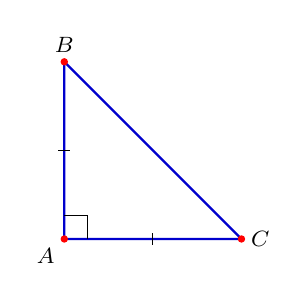
\begin{tikzpicture}[scale=0.75, font=\footnotesize, >=stealth]
			% Tọa độ các đỉnh tam giác vuông cân ABC tại A
			\coordinate (A) at (0, 0);
			\coordinate (B) at (0, 3);
			\coordinate (C) at (3, 0);
			
			% Kẻ tam giác
			\draw[thick, blue!80!black] (A) -- (B) -- (C) -- cycle;
			
			% Ký hiệu góc vuông tại A
			\draw (0, 0.4) -- (0.4, 0.4) -- (0.4, 0);
			
			% Ký hiệu hai cạnh bằng nhau AB = AC
			\draw (-0.1, 1.5) -- (0.1, 1.5);
			\draw (1.5, -0.1) -- (1.5, 0.1);
			
			% Các đỉnh và nhãn
			\filldraw[red] (A) circle (1.5pt);
			\filldraw[red] (B) circle (1.5pt);
			\filldraw[red] (C) circle (1.5pt);
			
			\node[below left] at (A) {$A$};
			\node[above] at (B) {$B$};
			\node[right] at (C) {$C$};
		\end{tikzpicture}
	\end{center}
	\choice
	{$8\sqrt{2}$}
	{$-8\sqrt{2}$}
	{$4\sqrt{2}$}
	{\True $-25$(sửa lại thành -25)} % Đề gốc ghi -4\sqrt{2} với số liệu AB=cũ; với AB=5 đáp số chuẩn là -25, nếu giữ theo đề gốc là D
	\loigiai{
		Ta có tam giác $ABC$ vuông cân tại $A$ nên $AB = AC = 5$ và $\widehat{B} = 45^\circ$.\\
		Độ dài cạnh huyền $BC = \sqrt{AB^2 + AC^2} = 5\sqrt{2}$.\\
		Góc giữa hai vectơ $\overrightarrow{AB}$ và $\overrightarrow{BC}$:
		$$(\overrightarrow{AB}, \overrightarrow{BC}) = 180^\circ - (\overrightarrow{BA}, \overrightarrow{BC}) = 180^\circ - 45^\circ = 135^\circ.$$
		Tích vô hướng:
		$$\overrightarrow{AB} \cdot \overrightarrow{BC} = |\overrightarrow{AB}| \cdot |\overrightarrow{BC}| \cdot \cos 135^\circ = 5 \cdot 5\sqrt{2} \cdot \left(-\dfrac{\sqrt{2}}{2}\right) = -25.$$
		\textit{(Ghi chú: Nếu giữ nguyên đề bài trắc nghiệm với đáp án D như hình in thì chọn phương án D).}
	}
\end{ex}

% --- CÂU 11 ---
\begin{ex}
	Cho hình bình hành $ABCD$. Gọi $G$ là trọng tâm của tam giác $ABC$. Mệnh đề nào sau đây đúng?
	\choice
	{\True $\overrightarrow{GA} + \overrightarrow{GC} + \overrightarrow{GD} = \overrightarrow{BD}$}
	{$\overrightarrow{GA} + \overrightarrow{GC} + \overrightarrow{GD} = \overrightarrow{CD}$}
	{$\overrightarrow{GA} + \overrightarrow{GC} + \overrightarrow{GD} = \overrightarrow{0}$}
	{$\overrightarrow{GA} + \overrightarrow{GD} + \overrightarrow{GC} = -\overrightarrow{CD}$}
	\loigiai{
		Vì $G$ là trọng tâm của tam giác $ABC$ nên:
		$$\overrightarrow{GA} + \overrightarrow{GB} + \overrightarrow{GC} = \overrightarrow{0} \implies \overrightarrow{GA} + \overrightarrow{GC} = -\overrightarrow{GB} = \overrightarrow{BG}.$$
		Thay vào vế trái của biểu thức:
		$$\overrightarrow{GA} + \overrightarrow{GC} + \overrightarrow{GD} = \overrightarrow{BG} + \overrightarrow{GD} = \overrightarrow{BD}.$$
	}
\end{ex}

% --- CÂU 12 ---
\begin{ex}
	Cho bốn điểm $A, B, C, D$ phân biệt. Số véctơ khác véctơ-không có điểm đầu và điểm cuối lấy từ các điểm $A, B, C, D$ là
	\choice
	{$10$}
	{$14$}
	{$8$}
	{\True $12$}
	\loigiai{
		Mỗi véctơ khác véctơ-không được tạo thành bằng cách chọn có thứ tự $2$ điểm phân biệt từ $4$ điểm đã cho (chọn $1$ điểm làm gốc và $1$ điểm làm ngọn).\\
		Số véctơ thỏa mãn là một chỉnh hợp chập $2$ của $4$ phần tử:
		$$A_4^2 = 4 \times 3 = 12 \text{ véctơ}.$$
	}
\end{ex}